\documentclass[journal]{IEEEtran}

\usepackage{graphicx}
\usepackage{booktabs}
\usepackage{amsmath}
\usepackage{textcomp}
\usepackage{url}
\usepackage{tikz}
\usetikzlibrary{arrows.meta,positioning}

\graphicspath{{../figures/}}

\begin{document}

\title{Recompiling Only What Changed: Matching-Based Incremental Recompilation for Modelica Digital Twins}

\author{Parth~Garg
\thanks{P. Garg is with Vellore Institute of Technology, Vellore, India (e-mail: parth.garg2024@vitstudent.ac.in).}}

\markboth{Preprint, to be reformatted for the target venue}{}

\maketitle

\begin{abstract}
A digital twin drifts out of sync when the machine it models changes structurally: a part is swapped, a sensor is added, a component is removed. Every simulation compiler we know of reacts by rebuilding the whole model from scratch, an outage a twin tracking a live system cannot always afford. We ask whether the compiled artifacts a localized structural edit actually invalidates are themselves localized, and build a pipeline that answers empirically rather than by assumption. We compute an equation-to-variable matching from a Modelica model's compiled differential-algebraic representation, partition it into recompilation units along the resulting block-lower-triangular structure, and resolve a change's impact by graph reachability from the equations it touched, never by diffing before and after. Every rebuilt binary is checked bit-identical against a full rebuild, never within a tolerance. On real Modelica-Standard-Library circuits we measure real, repeated speedups of 1.09$\times$--2.27$\times$; across a twentyfold model-size range the speedup holds in a 1.8$\times$--2.3$\times$ band rather than growing, because relinking, not recompiling, dominates incremental cost. Building the pipeline surfaced a non-deterministic third-party bipartite matcher and a quadratic bug in our own code generator, both found and fixed; we also measure an explicit break-even change frequency above which batching several edits beats recompiling after each one. We report where the approach stops working as plainly as where it works: models needing differential-index reduction, and scale beyond a few thousand equations, are both out of reach here.
\end{abstract}

\begin{IEEEkeywords}
Modelica, digital twins, incremental compilation, incremental recompilation, equation-based modeling, differential-algebraic equations, structural change, build systems.
\end{IEEEkeywords}

\section{Introduction}

A digital twin is only useful while it matches the machine it twins. Real machines change: a part is swapped, a sensor is added, a component is removed. When that happens the twin's simulation code should update too, but every tool we are aware of responds to a structural edit by rebuilding the whole model from scratch, slow enough to force the twin offline while it runs. General-purpose incremental build systems such as Make~\cite{feldman1979make} solved the analogous problem for source files decades ago; this paper asks whether the same idea transfers to equation-based simulation compilers, where the units of compilation are equations and the unknowns they solve for rather than files.

We build a pipeline that answers this empirically, using a real, actively developed Modelica compiler, Rumoca~\cite{condie2026rumoca}, and real Modelica Standard Library components. It computes its own equation-to-unknown matching from the compiler's exported intermediate representation (Rumoca does not expose its internal matching), defines a recompilation unit as one block of that matching's block-lower-triangular structure, and predicts which units a structural edit affects by graph reachability from the equations the edit touched, never by diffing the model before and after. Every incrementally rebuilt binary is required to match a from-scratch rebuild bit-for-bit, and that requirement is checked on every measured cell, not asserted once.

The result is a genuine but narrow positive finding, reported with its limitations attached rather than around them: incremental recompilation is measurably faster on real circuits, the speedup does not grow with model size under the current relink-everything design, and generality stops at models needing differential-index reduction. Section~\ref{sec:background} reviews Modelica compilation and incremental build systems; Section~\ref{sec:method} describes the pipeline; Section~\ref{sec:results} reports every measurement; Sections~\ref{sec:limitations}--\ref{sec:future} state what remains open.

\section{Background and Related Work}
\label{sec:background}

\subsection{Digital twins and drift}

The term digital twin traces to Grieves' manufacturing white paper~\cite{grieves2014twin}, describing a virtual representation kept synchronized with a physical asset. Recent model-driven-engineering work names this synchronization problem directly: Abbasi et al.~\cite{abbasi2024drift} formalize semantic drift in model-driven digital twins and argue that reacting to structural, not only parameter, drift is largely open. We do not attempt to detect structural change; every edit in our experiments is injected by a script that already knows exactly which equations it touched. Our contribution is one step downstream: once a change is known, how much of the compiled model needs regenerating, and how fast.

\subsection{Modelica compilation}

Modelica compilers, including OpenModelica~\cite{fritzson2005openmodelica} and the newer MLIR-based MARCO~\cite{agosta2023marco}, flatten a hierarchical model into a flat differential-algebraic system, match each equation to an unknown, decompose the matched system into block-lower-triangular (BLT) form so blocks solve in dependency order, and generate code, typically one routine per block. MARCO reports simulating models with millions of equations in tens of seconds, a useful reference for how fast a full rebuild already is at scale. A BLT block is a natural but not identical candidate for a recompilation boundary, since it reflects simultaneous-solve requirements rather than the read/write dependency between generated code; Section~\ref{sec:method} describes the correction this required. Some Modelica compilers additionally perform differential-index reduction (Pantelides' algorithm~\cite{pantelides1988consistent}) to causalize models with purely reactive loops, a step our own matcher does not attempt to replicate (Section~\ref{sec:limitations}).

Our front end is Rumoca~\cite{condie2026rumoca}, a Rust-native Modelica compiler, used through its Python bindings to obtain a model's compiled DAE representation as JSON. Its public API does not expose the internal matching or BLT structure, so the matcher used throughout this paper is a from-scratch implementation (Section~\ref{sec:matching}). We do not build on the Functional Mock-up Interface~\cite{blochwitz2012fmi}, the Modelica ecosystem's tool-independent model-exchange standard, since it packages a model as an opaque binary unit for co-simulation; recompiling only part of that unit needs direct control over per-equation code generation, which an FMU boundary does not expose.

\subsection{Incremental build systems}

Make~\cite{feldman1979make} tracks dependencies between source and object files and rebuilds only targets whose inputs changed; modern successors such as Bazel generalize the idea with a content-addressed, hermetic dependency graph. The mapping here is direct: an equation plays the role of a source file, a recompilation unit plays the role of a compiled object, and the equation-variable dependency graph plays the role of the build graph. What differs is that this dependency graph is not handed to us the way \texttt{\#include} directives are; it must be derived from the compiler's own matching, which a general-purpose build system never has to compute.

\section{Method}
\label{sec:method}

\subsection{Pipeline overview}

Each experiment cell runs five stages: compile the model; compute the matching and recompilation-unit partition; inject a structural change into the source and recompile the changed model independently; resolve the change's impact by graph reachability on the changed model's own dependency graph; and recompile only the predicted units, relink against cached objects for the rest, and compare against a full rebuild. Fig.~\ref{fig:pipeline} summarizes the flow. Only the first stage is Rumoca itself; every later stage is our own code.

\begin{figure}[!t]
\centering
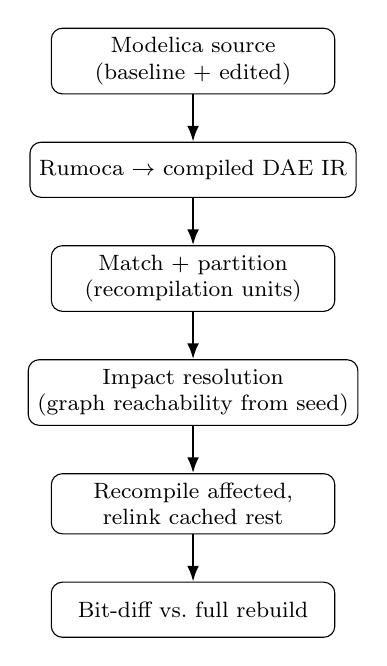
\begin{tikzpicture}[
  node distance=6mm and 6mm,
  box/.style={draw, rounded corners, align=center, minimum width=3.6cm, minimum height=7mm, font=\footnotesize},
  arr/.style={-{Latex[length=2mm]}, thick}
]
\node[box] (src) {Modelica source\\(baseline + edited)};
\node[box, below=of src] (ir) {Rumoca $\to$ compiled DAE IR};
\node[box, below=of ir] (match) {Match + partition\\(recompilation units)};
\node[box, below=of match] (resolve) {Impact resolution\\(graph reachability from seed)};
\node[box, below=of resolve] (build) {Recompile affected,\\relink cached rest};
\node[box, below=of build] (check) {Bit-diff vs.\ full rebuild};
\draw[arr] (src) -- (ir);
\draw[arr] (ir) -- (match);
\draw[arr] (match) -- (resolve);
\draw[arr] (resolve) -- (build);
\draw[arr] (build) -- (check);
\end{tikzpicture}
\caption{The five-stage pipeline used for every experiment cell.}
\label{fig:pipeline}
\end{figure}

\subsection{Sourcing the matching}
\label{sec:matching}

Let $E$ be the equation set and $V$ the unknown set of a well-posed square DAE system, $|E|=|V|$, with an incidence relation pairing equation $e$ with variable $v$ whenever $e$'s residual depends on $v$. A perfect matching pairs every equation with a distinct variable respecting that incidence, i.e., a maximum matching on the resulting bipartite incidence graph. We originally planned to extract Rumoca's own internally computed matching, since it clearly computes one to compile any model with implicit equations, but its public API exposes only the flattened stage, not the matched one. We built a from-scratch matcher instead, verified against Rumoca's own block-count statistics on every model tested, including a real 69-equation Modelica-Standard-Library circuit.

Building it surfaced two bugs. A greedy two-pass strategy, assigning each equation its syntactically obvious target before augmenting-path search, can strand an equation even when a valid perfect matching exists overall; we replaced it with one full bipartite-matching pass. More seriously, \texttt{networkx}'s Hopcroft--Karp implementation~\cite{hopcroft1973n52} was non-deterministic across process runs on one real graph: identical input produced different matchings, traced to Python's per-process hash randomization leaking into its traversal order. We replaced it with a hand-rolled augmenting-path (Kuhn's) matcher~\cite{kuhn1955hungarian}, verified deterministic across twenty in-process runs and five independent subprocesses under five different hash seeds.

\subsection{Recompilation unit definition}

Given the matching $M$, define a directed graph $G_M=(E,A)$ with an arc $e_i \to e_j$ whenever equation $e_j$'s residual reads $M(e_i)$. A recompilation unit is the equation membership of one strongly connected component of $G_M$~\cite{tarjan1972depth}, equivalently one block of the matched system's block-triangular form~\cite{duff1978implementation}: equations $e_i,e_j$ share a unit exactly when a directed cycle in $G_M$ contains both.

One correction mattered in practice. Treating a state variable as an ordinary read/write target manufactures cycles a real solver never has: an explicit ODE's derivative equation reads its own state, and if some algebraic variable is itself a function of that state, the raw graph sees a cycle even though a numerical solver evaluates the two directly, never iterating between them. On an early three-room thermal-network fixture this collapsed eight of nine equations into one unit despite a simple nearest-neighbor topology. Excluding states as edge sources, since a state is a known each timestep rather than something solved jointly with the algebraic system, removed the artifact and reduced the same model to nine correctly matched units, agreeing exactly with the compiler's own block count.

\subsection{Change injection, impact resolution, and soundness}

Every structural change is a literal text-level edit to the Modelica source (a component swap, sensor addition, or removal), recompiled through the same front end as any other model. Impact resolution takes the seed set, the equations the injector directly edited, and follows dependency edges outward on the changed model's post-change graph, purely by reachability; it never inspects a before/after diff, so it cannot benefit from already knowing the answer it is checked against.

That check is independent: we diff the baseline and changed model's compiled equations directly (stripping source-position metadata) and confirm the resolver's predicted set is a superset of every equation that actually changed. This passed with no missed units on every cell measured, and a dedicated test confirms the check has teeth: a detector given an empty seed set is correctly flagged unsound, with the missed unit named.

\subsection{Code generation and incremental build}

Each unit becomes its own C translation unit. For a singleton unit matched to unknown $x$, the residual $r(x)=0$ is extracted into affine form $r(x)=ax+b$ over that unit's own unknown, solved as $x=-b/a$. For a coupled unit with unknowns $x_1,\dots,x_k$, stacking one row per member equation gives a linear system $A\mathbf{x}=\mathbf{b}$, solved with a shared, size-parameterized Gaussian-elimination routine with partial pivoting. Both paths share the same affine-extraction code; an earlier version of the singleton path assumed a matched variable always sits alone on one side of its equation as written, false whenever the matcher assigns an equation to a variable other than its syntactic left-hand side, which produced a real, silent, self-referential wrong assignment on one Modelica-Standard-Library resistor model until unified onto one provably correct path.

A full rebuild compiles and links every unit; an incremental rebuild recompiles only the resolver's affected units, copies cached objects for the rest, and relinks the complete set. Every reused object's SHA-256 hash is checked against its cached baseline, and every measured cell additionally requires the two binaries' simulation output to match exactly, either at zero absolute error or, for larger models, by literal string equality of the full printed trace, a strictly stronger check than a numeric tolerance. No tolerance was invoked to pass a result in this paper.

\section{Experimental Setup}
\label{sec:setup}

All experiments ran on one Windows machine using Rumoca~0.9.20 through its Python bindings, Python~3.11.9, and MinGW-w64 GCC~15.2, with every compile and link step timed as a real subprocess call, never derived from another timing by arithmetic. Two model families are used: real circuits built from genuine \texttt{connect()}-wired Modelica Standard Library components, and a parameterized thermal-chain generator producing an $N$-room model with $3N{-}1$ equations on the same index-1 topology validated in Section~\ref{sec:method}, used to test how the approach behaves as size grows beyond what any single hand-written model covers. Table~\ref{tab:models} lists both. All code, models, and logs are in the project repository; every number below cites the script and log it came from.

\begin{table}[!t]
\caption{Models used in the experiments.}
\label{tab:models}
\centering
\footnotesize
\begin{tabular}{lccl}
\toprule
Model & Eqns.\ & Units & Role \\
\midrule
MslRcCircuit & 23 & 23 & Real MSL, swap/sensor \\
MslResistorNetwork & 35 & 22 & Real MSL, removal \\
CauerLowPassAnalog & 69 & 67/69 & Real MSL, negative result \\
ThermalChain($N$) & $3N{-}1$ & $3N{-}1$ & Generated, scale sweep \\
\bottomrule
\end{tabular}
\end{table}

\section{Results}
\label{sec:results}

We report measured speedup as $S=T_\text{full}/T_\text{incr}$, the ratio of mean full to mean incremental rebuild time, and ripple as $\rho=U_\text{aff}/U_\text{tot}$, the affected fraction of recompilation units; neither is ever derived by projecting the other.

\subsection{Generality on real Modelica-Standard-Library models}
\label{sec:msl-results}

Table~\ref{tab:msl-speedup} and Fig.~\ref{fig:msl-speedup} report measured, five-times-repeated speedup for three change cells. Every cell is bit-identical to a full rebuild and every reused object byte-identical to its cache.

\begin{table}[!t]
\caption{Measured speedup on real MSL models.}
\label{tab:msl-speedup}
\centering
\footnotesize
\begin{tabular}{lccc}
\toprule
Change & Units affected & Full & Incr. \\
\midrule
Resistor $\rightarrow$ Conductor & 13/23 & 552.9 ms & 506.3 ms \\
Sensor addition & 1/24 & 595.9 ms & 382.1 ms \\
Resistor removal & 11/18 & 589.3 ms & 437.5 ms \\
\bottomrule
\end{tabular}
\end{table}

\begin{figure}[!t]
\centering
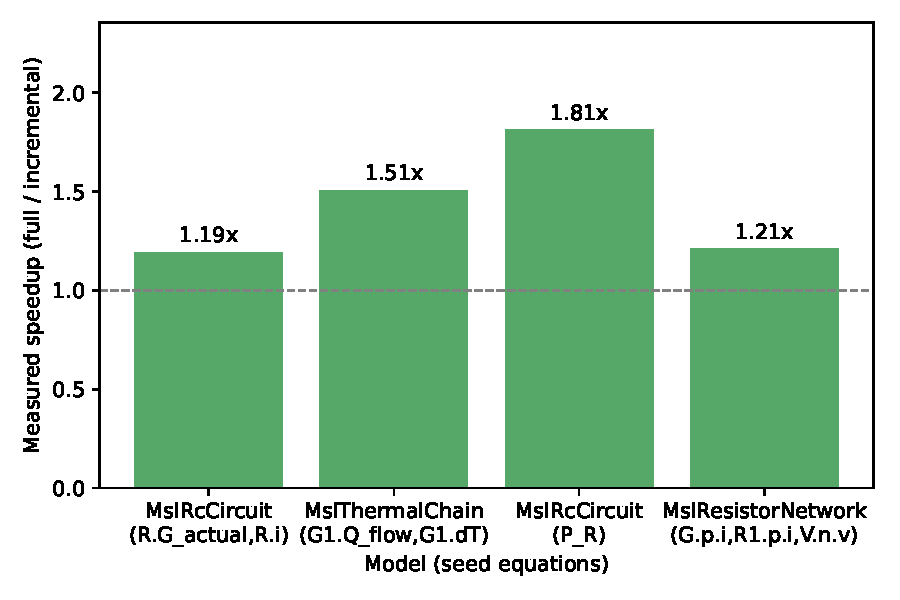
\includegraphics[width=0.95\linewidth]{measured_speedup.pdf}
\caption{Measured speedup, real MSL models.}
\label{fig:msl-speedup}
\end{figure}

\begin{figure}[!t]
\centering
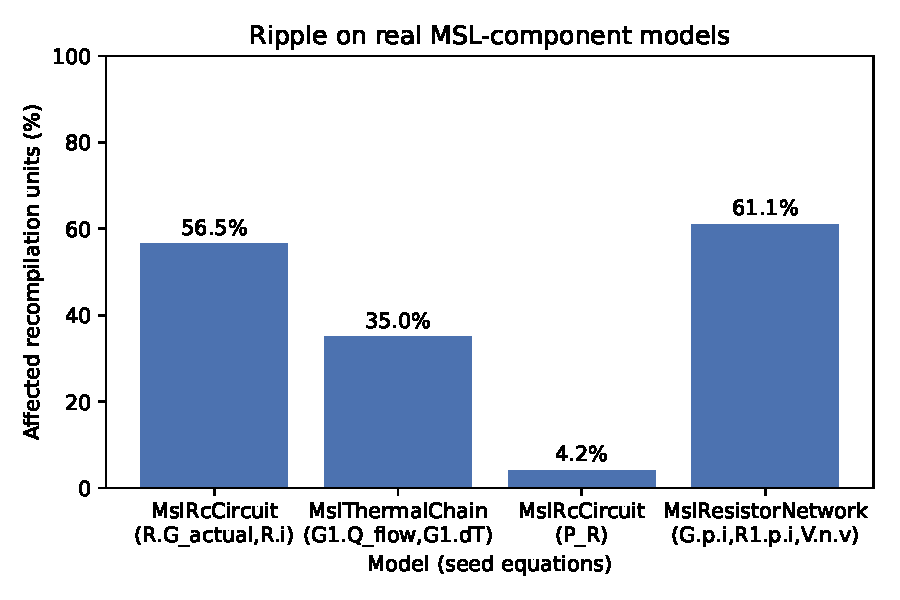
\includegraphics[width=0.95\linewidth]{real_model_ripple.pdf}
\caption{Ripple $\rho$ per change, real MSL models.}
\label{fig:ripple}
\end{figure}

Speedup ranges 1.09$\times$--1.56$\times$, with $\rho$ (Fig.~\ref{fig:ripple}) ranging 4\%--61\% and showing no simple relationship to speedup: the sensor-addition cell has both the smallest $\rho$ and the largest speedup, as expected, but resistor removal has the largest $\rho$ of the three (61\%, higher than the resistor swap's 57\%) while still beating the resistor swap's speedup, because at this model size wall-clock speedup depends on more than $\rho$ alone, as the timing variance discussed next shows directly. We disclose directly that these particular numbers are noisier across independent re-runs than expected: on models with only 23--24 total units, fixed compiler/linker process-spawn overhead is large relative to the work saved, so four separate re-runs of the identical script and code varied by up to roughly 30--40\% relative to each other, while $\rho$ stayed exactly identical every time, confirming the matching and resolution logic is deterministic and only wall-clock timing on tiny builds is noisy. Section~\ref{sec:scale-results}'s larger sweep is the more statistically stable claim.

\subsection{A genuine scaling defect: quadratic code generation}
\label{sec:on2}

Profiling ahead of the scaling experiments below found our code generator, not the matcher, partitioner, or graph builder (all near-linear), scaled quadratically (Table~\ref{tab:on2}).

\begin{table}[!t]
\caption{Codegen time before/after the fix (Sec.~\ref{sec:on2}).}
\label{tab:on2}
\centering
\footnotesize
\begin{tabular}{lccc}
\toprule
Equations & Before & After & Speedup \\
\midrule
2{,}999 & 3.13 s & 0.37 s & 8.5$\times$ \\
14{,}999 & 88.86 s & 1.81 s & 49$\times$ \\
\bottomrule
\end{tabular}
\end{table}

A fivefold size increase cost 28.4$\times$ longer before the fix ($\log 28.4/\log 5 \approx 2.09$, quadratic). The cause: the per-unit emitter rebuilt a name-to-slot lookup table and linearly scanned for each variable's index once per unit inside a loop over all $N$ units, turning $O(N)$ per call into $O(N^2)$ overall. Replacing the scan with a dictionary built once per model changed only the lookup mechanism, confirmed by an unchanged regression suite; the same fivefold increase now costs 4.85$\times$ longer ($\log 4.85/\log 5 \approx 0.99$, linear).

\subsection{Speedup versus model size}
\label{sec:scale-results}

Table~\ref{tab:scale} and Fig.~\ref{fig:speedup-size} report measured, three-times-repeated speedup across a twentyfold size range, all cells bit-identical.

\begin{table}[!t]
\caption{Incremental speedup vs.\ model size.}
\label{tab:scale}
\centering
\footnotesize
\begin{tabular}{lccc}
\toprule
Equations & Full & Incr. & Speedup \\
\midrule
149    & 3.04 s  & 1.34 s  & 2.27$\times$ \\
299    & 5.44 s  & 2.90 s  & 1.88$\times$ \\
749    & 14.43 s & 7.02 s  & 2.05$\times$ \\
1{,}499 & 34.07 s & 16.02 s & 2.13$\times$ \\
2{,}999 & 72.18 s & 39.29 s & 1.84$\times$ \\
\bottomrule
\end{tabular}
\end{table}

\begin{figure}[!t]
\centering
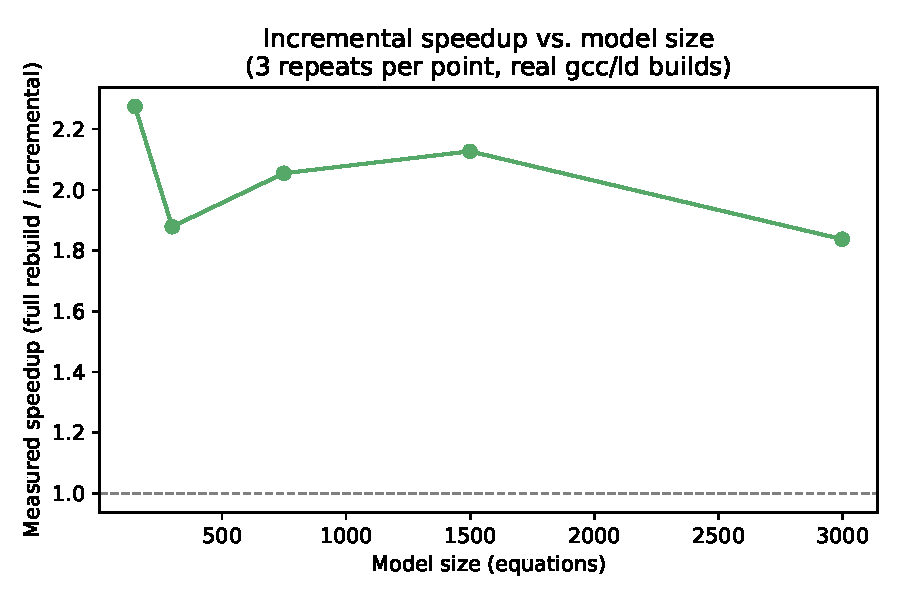
\includegraphics[width=0.95\linewidth]{speedup_vs_size.pdf}
\caption{Speedup vs.\ model size.}
\label{fig:speedup-size}
\end{figure}

Speedup stays in a 1.8$\times$--2.3$\times$ band instead of growing, though only 2 of every $3N{-}1$ units are ever affected, a shrinking fraction as $N$ grows. The cause is named, not just observed: our incremental rebuild always relinks every cached object, never only the changed delta. With recompilation near-instant at every size, relinking the full $3N{-}1$-object set is what the incremental build's time is spent on. Two facts support this: the incremental timing's relative standard deviation grows with size (30\% at $N{=}1{,}000$ vs.\ the full rebuild's 4\%, consistent with I/O-bound relink noise against CPU-bound recompile consistency), and an independent one-off at 1,499 equations with 99.87\% of units unaffected still took 11.3 s incrementally against a 29.8 s full rebuild, far short of the roughly 700$\times$ a ripple-proportional model would predict, because that 11.3 s is spent relinking 1,499 objects, not recompiling two files.

\subsection{One-time setup overhead versus model size}

The one-time cost of Rumoca's own parse plus our matching, partitioning, and graph construction stays a small, non-trending fraction of full-rebuild cost: 3.0\% at 149 equations, 5.2\% at 2,999 (Fig.~\ref{fig:overhead}). Standing the pipeline up on a given model does not become the bottleneck as it grows, at least across the tested range.

\begin{figure}[!t]
\centering
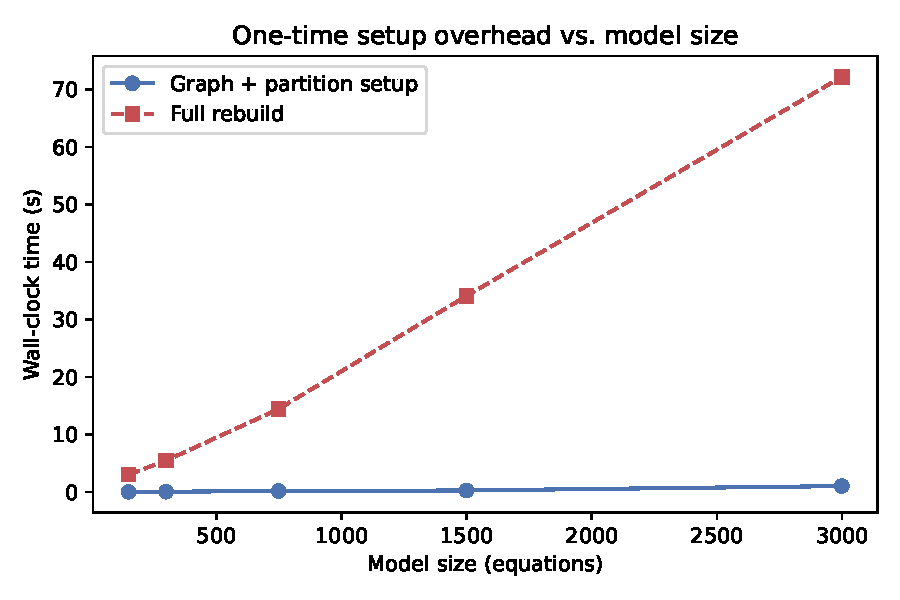
\includegraphics[width=0.95\linewidth]{overhead_vs_size.pdf}
\caption{Setup overhead vs.\ model size.}
\label{fig:overhead}
\end{figure}

\subsection{A measured break-even change frequency}

The operationally relevant question is not whether incremental recompilation ever wins in isolation, but whether, given how often changes actually arrive, it beats letting several accumulate before rebuilding. We drive a real, cumulative sequence of $K{=}10$ structural edits on an 899-equation model, each written atop the previous edit's already-edited source, through two strategies: streaming incremental (recompile and relink after every change) and batched full (accumulate, rebuild once every $B$ changes). Batching at size $B$ wins when
\[
\left\lceil K/B \right\rceil \, T_\text{full} \;<\; T_\text{stream}.
\]
The ten-change stream totaled $T_\text{stream}=63.0$ s; a directly measured, three-times-repeated $T_\text{full}=18.9$ s. Table~\ref{tab:breakeven} and Fig.~\ref{fig:breakeven} sweep $B$ against these two real numbers.

\begin{table}[!t]
\caption{Break-even sweep over batch size $B$.}
\label{tab:breakeven}
\centering
\footnotesize
\begin{tabular}{lccc}
\toprule
$B$ & Rebuilds & Batched total & Cheaper? \\
\midrule
1  & 10 & 189.3 s & No \\
2  & 5  & 94.7 s  & No \\
3  & 4  & 75.7 s  & No \\
\textbf{4}  & \textbf{3}  & \textbf{56.8 s}  & \textbf{Yes} \\
5  & 2  & 37.9 s  & Yes \\
10 & 1  & 18.9 s  & Yes \\
\bottomrule
\end{tabular}
\end{table}

\begin{figure}[!t]
\centering
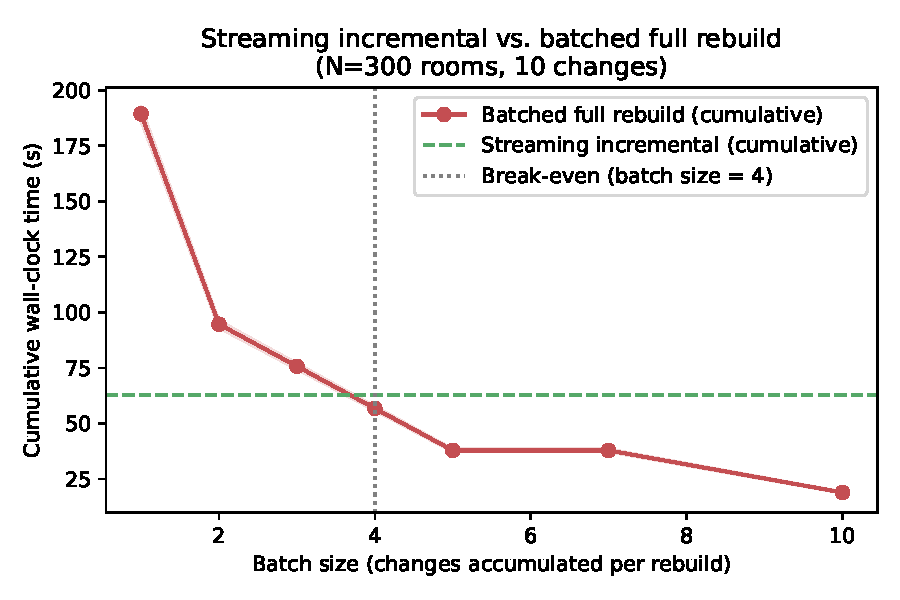
\includegraphics[width=0.95\linewidth]{break_even_crossing.pdf}
\caption{Streaming vs.\ batched cumulative cost.}
\label{fig:breakeven}
\end{figure}

Batching wins once four or more changes accumulate before a rebuild is due, stable even under the full-rebuild timing's own worst-case measured spread. We consider this the single most operationally useful number in the paper: it tells an operator the change frequency above which they should stop recompiling after every edit.

\section{Limitations and Threats to Validity}
\label{sec:limitations}

\emph{Scale.} The target was on the order of $10^5$ equations. The full pipeline has been verified bit-identical only to 1,499 equations; repeated speedup/overhead measurements reach 2,999; codegen was profiled, timing only, to 14,999; the compiler was asked to parse, compile only, at most 29,999. This is scoped deliberately: the front end's own parse time grows faster than linearly, and a repeated-measurement cell at $10^5$ equations was not affordable here. The reported trend (speedup holding steady, not growing) is a trend to 2,999 equations, never extrapolated further.

\emph{Index-1 models only.} Every validated model is index-1. A 69-equation Cauer filter with two independent capacitor-only loops needs genuine differential-index reduction~\cite{pantelides1988consistent} before causalization, which our matcher does not attempt; the two equations it cannot place are exactly the two potential-equality constraints closing those loops, confirming a genuine structural gap, not a matcher bug.

\emph{The relink ceiling.} Incremental rebuild always relinks every cached object, the direct, named cause of the plateau in Section~\ref{sec:scale-results}. A partial-link strategy, incremental linking or a shared-object boundary per unit, would likely raise it; not attempted here, since the matching and partitioning logic that would need to stay correct underneath it was the higher-risk part of this project's scope.

\emph{Linear coupled blocks only.} No tested model, real or hand-written, has a genuine nonlinear algebraic loop, so nonlinear (Newton-iteration) block codegen was never built.

\emph{No discrete or event-driven signals.} Standard MSL signal sources compile a start-time conditional our emitter cannot translate; worked around by choosing a different, still genuine swap.

\emph{Small-model timing variance.} As in Section~\ref{sec:msl-results}, models with only a few dozen units show large relative variance between re-runs, traced to process-spawn overhead. Section~\ref{sec:scale-results} is the more stable claim.

\emph{Change detection is out of scope.} Every change is injected by a script that already knows which equations it touched; detecting that a change happened is not addressed.

\emph{Small real-model corpus.} Generality is shown on two real circuits plus the Cauer filter as a negative result; a systematic characterization across a larger corpus was not attempted.

\section{Future Work}
\label{sec:future}

The highest-leverage next step is a partial or incremental link strategy, since relinking, not recompiling, is the current bottleneck at scale, and raising that ceiling likely needs no change to the matching or partitioning logic. Extending the matcher with differential-index reduction~\cite{pantelides1988consistent} would open the approach to models like the Cauer filter, structurally common wherever a purely reactive loop or cutset appears; adding Newton-iteration codegen would remove the linear-only restriction, though neither has been shown necessary by any model encountered here. Scaling further toward $10^5$ equations is gated mainly by the front end's superlinear compile time rather than this paper's own pipeline. Finally, the change-detection problem set aside here, identifying that a structural edit occurred and which equations it touched, is a natural companion to the impact-resolution machinery described above.

\section{Conclusion}
\label{sec:conclusion}

We built and measured, rather than merely proposed, a matching-based incremental recompilation pipeline for Modelica models, using a real compiler front end and real Modelica-Standard-Library components throughout. Incremental recompilation is measurably faster than a full rebuild, correctness holds exactly on every measured cell, and we report a concrete, measured break-even change frequency. At the same time, speedup does not grow with model size for a diagnosed and fixable reason, and generality stops precisely at models requiring differential-index reduction. Both results are reported at the same level of evidence: real, repeated, independently verified measurements, not projections.

\bibliographystyle{IEEEtran}
\bibliography{refs}

\end{document}
